\documentclass[11pt, a4paper]{scrartcl}

\usepackage{listings}
\usepackage{jlcode}
\usepackage{color}
\usepackage[utf8]{inputenc}
\usepackage{hyperref}
\usepackage{graphicx}
\usepackage{float}

\title{Julia Installationsanleitung für Windows}
\author{}
\date{}

\definecolor{dkgreen}{rgb}{0,0.6,0}
\definecolor{dkblue}{rgb}{0,0,0.4}
\definecolor{gray}{rgb}{0.5,0.5,0.5}
\definecolor{mauve}{rgb}{0.58,0,0.82}

\hypersetup{
	colorlinks=true,
	linkcolor=black,
	urlcolor=dkblue,
}
\lstset{
	language=Julia,
	%	frame=tb,
	aboveskip=3mm,
	belowskip=3mm,
	showstringspaces=false,
	columns=flexible,
	basicstyle={\small\ttfamily},
	numbers=none,
	numberstyle=\tiny\color{gray},
	keywordstyle=\color{blue},
	commentstyle=\color{dkgreen},
	stringstyle=\color{mauve},
	breaklines=true,
	breakatwhitespace=true,
	tabsize=3
}



\begin{document}
%\maketitle

\section{IJulia Error}

Nach der Installation von $IJulia$ wird von $notebook()$ kein Notebook geöffnet. In manchen Fällen schlägt $Pkg.add("IJulia")$ fehl. (Build error von ZMQ und MbedTLS)

\begin{lstlisting}
	julia> using IJulia
	julia> notebook()
	[ Info: running setenv(...)
	Process(setenv(...), ProcessExited(1))
\end{lstlisting}


\section{Lösung 1: Anaconda}

Anaconda ist eine Python Umgebung, die Jupyter Notebooks beinhaltet. Sie können diese als Alternative zu IJulia benutzen. Laden Sie Anaconda für Python 3.7 von \url{https://www.anaconda.com/distribution/} herunter. (Achtung: macOS ist als Standard ausgewählt)

\begin{figure}[h!]
	\centering
	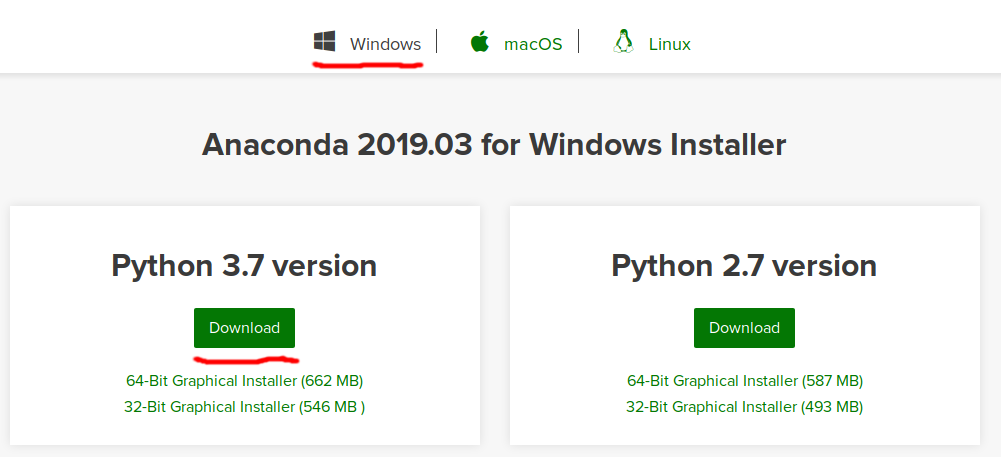
\includegraphics[width=0.6\textwidth]{img/download.png}
\end{figure}

Führen Sie die heruntergeladene Datei aus um Anacodna zu installieren. "Micorsoft VSCode" brauchen Sie dabei nicht zu installieren.

\begin{figure}[H]
	\centering
	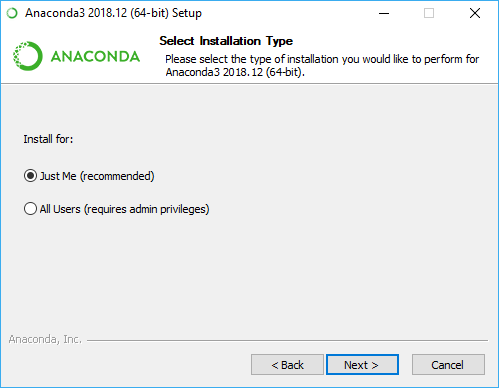
\includegraphics[width=0.4\textwidth]{img/install1.png}
	\vspace{0.1\textwidth}
	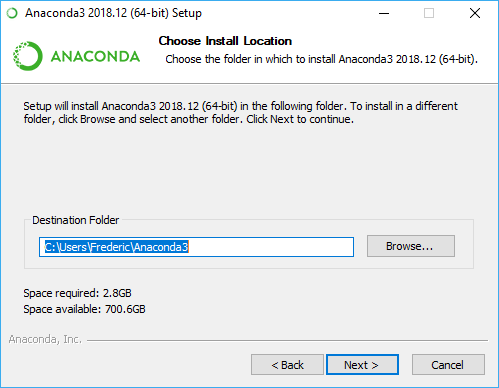
\includegraphics[width=0.4\textwidth]{img/install2.png}
\end{figure}

\begin{figure}[H]
	\centering
	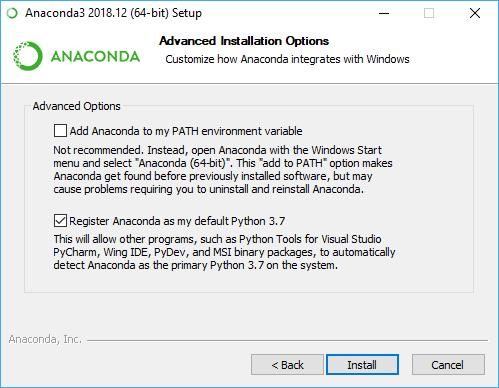
\includegraphics[width=0.4\textwidth]{img/install3.png}
	\vspace{0.1\textwidth}
	
\includegraphics[width=0.4\textwidth]{img/install4.png}
\end{figure}

Nach der Installation sollte "Jupyter Notebook" unter "Anaconda3" im Startmenü verfügbar sein.

Falls die Installation von $IJulia$ bis auf das öffnen der Notebooks mit $notebook()$ funktioniert hat, sollte Julia in Jupyter Notebooks verfügbar sein. Prüfen Sie dieses indem Sie das Jupyter Notebook über das Startmenü öffnen. Es sollte sich ein neuer Tab in ihren Webbrowser öffnen. Auf der rechten Seite sollte unter "New" ihre Julia Version verfügbar sein.

\begin{figure}[h!]
	\centering
	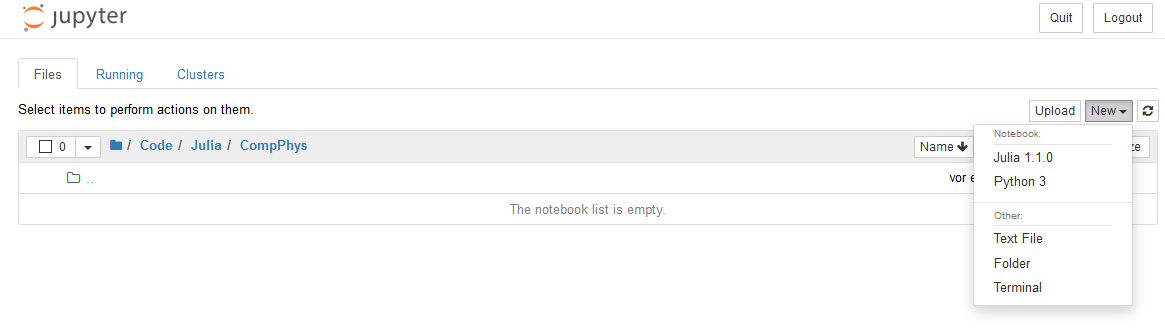
\includegraphics[width=0.8\textwidth]{img/notebook.png}
\end{figure}

Ist dies nicht der Fall, versuchen Sie $IJulia$ erneut zu installieren. Falls $Pkg.add("IJulia")$ fehlschlägt, müssen Sie dafür $Julia$ im Administratormodus ausführen. (Rechtsklick, Als Administrator ausführen) Sie können $IJulia$ mit 
\begin{lstlisting}
	using Pkg
	Pkg.rm("IJulia")
	Pkg.gc()
\end{lstlisting}
deinstallieren.\textbf{}


\newpage
\section{Lösung 2: Python löschen}


Deinstallieren Sie alle Python Distributionen (Python2.x, Python3.x, Anaconda, Conda, Canopy, ...) und IJulia ($Pkg.rm("IJulia"); Pkg.gc()$). Löschen Sie dann die Ordner
\begin{itemize}
	\item "C:\textbackslash Users\textbackslash \{Benutzername\}\textbackslash .julia\textbackslash conda"
	\item "C:\textbackslash Users\textbackslash \{Benutzername\}\textbackslash .conda"
\end{itemize}
sowie alle Ordner die direkt mit Python zu tun haben (Jupyter, Python, Conda, Anaconda, ...) unter 
\begin{itemize}
	\item "C:\textbackslash Users\textbackslash \{Benutzername\}\textbackslash AppData\textbackslash local"
	\item "C:\textbackslash Users\textbackslash \{Benutzername\}\textbackslash AppData\textbackslash roaming"
\end{itemize}
Sie können den Ordner "...\textbackslash AppData\textbackslash roaming" über "\%AppData\%" in der Adressleiste erreichen. Nachdem Sie alle Ordner gelöscht haben, installieren Sie IJulia erneut wie in der Anleitung beschrieben


\end{document}